\documentclass[11pt]{article}

%imports
\usepackage[utf8]{inputenc}
\usepackage[T1]{fontenc}
\usepackage{amsmath}
\usepackage{amsfonts}
\usepackage{amssymb}
\usepackage{footnote}
\usepackage{url}
\usepackage{hyperref}
\usepackage{subcaption}
\usepackage{tikz}
\usepackage{amsthm}
\usepackage{longtable}
\usepackage{float}

\usetikzlibrary{fit,shapes.geometric}


%images and image path
\usepackage{graphicx}
\graphicspath{ {./images/} }

%custom commands
\newcommand{\R}{\mathbf{R}}
\newcommand{\C}{\mathbf{C}}
\newcommand{\N}{\mathcal{N}}
\newcommand{\num}{\text{num}}
\newcommand{\obs}{\text{obs}}
\newcommand{\D}{\mathfrak{D}}
\newcommand{\Ro}{\mathcal{R}_0}
\newcommand{\lap}{{\mathcal{L}}}
\renewcommand\vec{\mathbf}
\newcommand{\mat}[1]{\mathsf{#1}}
\newcommand{\U}{\mathcal{U}}

\newtheorem{theorem}{Theorem}
\newtheorem{conjecture}{Conjecture}
\newtheorem{definition}{Definition}

%intsitute command
\usepackage{etoolbox}
\makeatletter
\providecommand{\institute}[1]{% add institute to \maketitle
	\apptocmd{\@author}{\end{tabular}
	\par
	\begin{tabular}[t]{c}
		\small \textit{#1}}{}{}
}
\makeatother

%margins
\usepackage[letterpaper, total={6.5in, 9.5in}]{geometry}

%opening
\title{Reaction-diffusion spatial modeling of COVID-19 in Chicago}
\author{Trent Gerew\thanks{\texttt{tgerew@hawk.iit.edu}}}
\institute{Department of Applied Mathematics, Illinois Institute of Technology, Chicago, Illinois}

\begin{document}

\maketitle

\begin{abstract}
	We investigate whether a reaction-diffusion model considering only meanly daily movement is sufficient to describe the spread of the COVID-19 virus in Chicago.
	The model is calibrated using publicly available health data published by the city.
	We first study the system of partial differential equations, then derive the basic reproduction number $\Ro$.
	Then we consider the numerical simulations conducted from March 18 to June 24, 2020.
	Finally, we discuss shortcomings of the model, and offer some potential solutions.
\end{abstract}

\section{Introduction}
	Emerging from Wuhan, China in late 2019, the COVID-19 virus rapidly spread throughout the globe \cite{covid-name}.
	Since the outbreak, governments everywhere have been desperately trying to contain the pandemic.
	Now, with safe and effective vaccines being distributed, it is hoped the pandemic can be overcome \cite{vaccine}.
	Before the introduction of the vaccines, so-called ``non-therapeutic'' interventions \cite{interventions1} were frequently deployed.
	Prominent among these are social distancing, self quarantining, lockdowns, gathering limitations, and the use of personal protective equipment.
	Now with the Omicron variant on the rise \cite{omicron}, these interventions are once again becoming prominent with some European countries reintroducing lockdowns and travel restrictions \cite{lockdowns}.
	
	Many mathematical models have been proposed to study the spread of the virus.
	Most are compartment models, where a population is divided into groups according to the state of individuals.
	These are generally known as SIR type models.
	The majority of such models ignore any spatial components.
	\cite{s+t+spain} employs a SAIR model and includes mobility terms based on the position of cell phones to model the propagation of the disease through Spain.
	Similarly, \cite{Danon2020.02.12.20022566} incorporates daily movements into an SEIR model.
	In a different approach, \cite{giuliani2020modelling} considers a statistical model to handle diffusion of COVID-19 in Italy.
	
	Here, we follow \cite{Kevrekidis-2021} and \cite{Mammeri+2020+102+113} in building a virus model where the spatial propagation is modeled by a diffusion and the reactions are derived from an SAIR model.
	Specifically, we examine the spread of COVID-19 in the city of Chicago.
	Does a reaction-diffusion model, which considers only the average daily movements of the population, correctly describe the spread of the virus in Chicago?
	If it does, we can use the model to assess possible vaccination strategies or reopening scenarios.
	
	The paper is organized as follows.
	Section 2 outlines the methodology, including data collection, modeling assumptions, and parameter estimates.
	Section 3 contains a brief analysis of the model and the results.
	In Section 4, we offer a discussion of the shortcomings of the model, and how they can be improved.

\section{Materials and methods}
	\subsection{Confirmed and death data}
		In this study, we used the publicly available data sets of COVID-19 metrics provided by the City of Chicago Data Portal.
		\cite{Chicago-cases} includes daily counts of city-wide confirmed infected cases, hospitalizations, and deaths.
		Weekly cases, tests and deaths by ZIP code are logged in \cite{Chicago-zips}.
	
	\subsection{Mathematical model}
		We focus our study on four components of the epidemic flow (Figure \ref{fig:model}).
		That is, the populations of Susceptible individuals ($S$), Asymptomatic infected individuals ($A$), symptomatic Infected individuals ($I$), and Removed individuals ($R$).
		\begin{figure}[h]
			\centering
			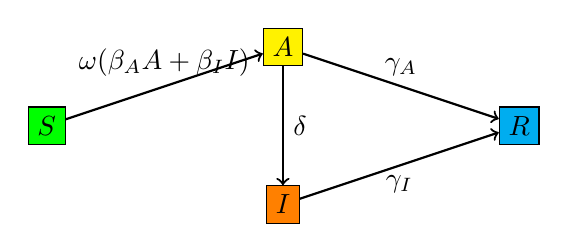
\begin{tikzpicture}
				\node[shape=rectangle, draw=black, fill=green] (s) at (-3,0) {$S$};
				\node[shape=rectangle, draw=black, fill=yellow] (a) at (0,1) {$A$};
				\node[shape=rectangle, draw=black, fill=orange] (i) at (0,-1) {$I$};
				\node[shape=rectangle, draw=black, fill=cyan] (r) at (3,0) {$R$};
				\path[thick,->] (s) edge node[above,swap] {$\omega (\beta_A A + \beta_I I)$} (a);
				\path[thick,->] (a) edge node[right,swap] {$\delta$} (i);
				\path[thick,->] (a) edge node[above,swap] {$\gamma_A$}	(r);
				\path[thick,->] (i) edge node[below,swap] {$\gamma_I$}	(r);
			\end{tikzpicture}
			\caption{Compartmental representation of the SAIR model.}
			\label{fig:model}
		\end{figure}
		Our model is known as the SAIR model \cite{s+t+spain}, which substitutes the $E$ compartment of the SEIR model by the $A$ compartment.
		This model is relevant when there are many undetected asymptomatic infectious individuals, which is known to be the case for COVID-19.
		
		A few notes motivating this very simple model are necessary.
		\begin{itemize}
			\item
				We do not consider the ``exposed'' $E$ group in this work.
				Because the members of $A$ have separate infection and recovery rates, and because there is a possibility they are detected and move to $I$, we consider $E$ to be merged with $A$.
			\item
				We do not distinguish between quarantined, hospitalized, or nursing home populations.
				Nursing homes are now known to be epicenters of the virus, however the true case rates are notoriously difficult to track \cite{nursing-homes}.
				Additionally, these three population groups can be assumed to be stationary in nature, and in the case of quarantined and hospitalized, isolated.
				Therefore we ignore their individual contributions.
			\item
				In general, the way in which data has been collected and is provided by authorities has varied over time, making its usage rather difficult\footnote{For an in-depth analysis of the data collection problem, see \cite{sara-soremo}.} \cite{messy-data1}, \cite{messy-data2}, \cite{challenges}.
				There is also the question of case counts being influenced by access to testing, especially early in the pandemic.
				Including additional compartments would over-parameterize the model making it more difficult to verify, and would not provide useful information.
			\item
				Lastly, adding additional compartments and parameters reduces the computational feasibility of the optimization problem.
		\end{itemize}
		The goal of this model is to strike a reasonable balance between representation of the pandemic and the populations involved, and feasibility of data collection and computation.
	
		To build the mathematical model, we followed the standard strategy developed in the literature concerning SIR models \cite{bio-models}.
		We assume that individuals in $S$ can be infected by both members of $A$ and $I$.
		We suppose that the individuals in the $A$ and $I$ compartments may have different contact rates $\beta_A$ and $\beta_I$, and different recovery rates $\gamma_A$ and $\gamma_I$.
		Furthermore, we consider a rate $\delta$ at which individuals in $A$ may develop symptoms or are otherwise detected and so will move to the $I$ compartment.
		Lastly, we assume that only members of $S$ and $A$ are mobile.
		
		The dynamics is governed by a system of two partial differential equations (PDE) and two ordinary differential equations (ODE) as follows, for $\vec{x} = (x,y) \in \Omega \subset \R^2, t > 0$,
		\begin{equation} \label{eq:model}
			\begin{aligned}
				S_t - D(t) \Delta S &= - \omega(t) \left( \beta_A A + \beta_I I \right) S, \\
				A_t - D(t) \Delta A &= \omega(t) \left( \beta_A A + \beta_I I \right) S - (\gamma_A - \delta) A, \\
				I_t &= - \gamma_I I + \delta A, \\
				R_t &= \gamma_A A + \gamma_I.
			\end{aligned}
		\end{equation}
		Since travel into the city of Chicago was heavily restricted for the early stages of the pandemic, the homogeneous Neumann boundary condition is imposed \cite{Mammeri+2020+102+113}.
		The population compartments are considered fractions, such that $S + A + I + R = 1$.
	
	\subsection{Parameter estimation}
		To account for the lockdown, the average number of of contacts is updated as in  \cite{Kevrekidis-2021}
		\begin{equation} \label{eq:contacts}
			\omega (t) = \omega_0 \left[ \eta + (1 - \eta) \frac{1 - \tanh \left[2 (t - t_q) \right]}{2} \right].
		\end{equation}
		Here, $t_q = (t_{\mathrm{eol}} + t_{\mathrm{bol}}) / 5$, where $\mathrm{bol}$ denotes the beginning of the lockdown and $\mathrm{eol}$ denotes the end of the lockdown.
		The parameter $0 \leq \eta \leq 1$ is a varying coefficient translating respect for social distancing and other preventative measures.
		Note that $\omega_0$ is the average number of contacts before any intervention, and is a constant.
		
		The parameters $\omega_0$, $\beta_A$, and $\beta_I$ are not independently identifiable, so the optimization problem reduces to five parameters $\theta = (\omega_0 \beta_A, \omega_0 \beta_I, \delta, \gamma_A, \gamma_I)$.
		Given, for $n$ days, the observations $I_\mathrm{obs} (t_i)$, the objective function is the least square function
		\begin{equation} \label{eq:obj}
			J (\theta) = \sum_{i=1}^n \left[ I_\mathrm{obs} (t_i) - I (t_i) \right]^2
		\end{equation}
		with constraints $0 \leq \theta \leq 1$.
		$I (t_i)$ denotes the output of the mathematical model at time $t_i$ computed with parameters $\theta$.
		
		The optimization problem is solved using the MATLAB nonlinear optimization function \verb|fmincon|.
		The initial parameter guesses to seed \verb|fmincon| were randomly sampled from a uniform distribution over 1000 iterations.
		The median of each resulting parameter was selected.
		Figure \ref{fig:params} shows the estimated parameters.
		
		The diffusion coefficient is also assumed to be altered by the lockdown, and is updated as a simple step function
			\begin{equation} \label{eq:diffusion}
				D(t) = D_0 \left[ 1 - (1 - \eta) H (t - t_\mathrm{bol}) \right]
			\end{equation}
		where $H(t)$ is the Heaviside step function.
		The average one-way commute in Chicago is about 5 miles \cite{travel}.
		Thus we set the diffusion coefficient $D_0$ to the fixed value of $5 / 0.72$ to convert to the spacing used for the discretization.
	
	\subsection{Numerical discretization}
		From the map of the city, the computational domain $\Omega$ is defined as the minimum square enclosing the city.
		The city is contained by $\Omega' = \left\{ (X,Y) \mid X \in [-87.9397, -87.5245], \ Y \in [41.6447, 42.023] \right\}$ where $X$ represents degrees latitude and $Y$ represents degrees longitude.
		Note that degrees latitude and longitude are not equal when converted to miles.
		Therefore, we define the computational domain such that the grid spacing is approximately 0.72 miles in both axes.
		This gives the domain
		\begin{equation} \label{eq:domain}
			\Omega = \left\{ \vec{x} \in \R^2 \mid x \in [0, 40], \ y \in [0, 29] \right\}.
		\end{equation}
		
		The initial spatial distribution of the infected population is determined by sampling the ZIP code data of confirmed cases \cite{Chicago-zips} at the grid points, as shown in Figure \ref{fig:seeding}.
		
		The model is solved via finite differences, using the \verb|scikit-fdiff| Python module \cite{nicolas_cellier_2019_3236970}.
		It is important to note that due to the limitations of the solver, the simulation had to be broken into time blocks where the values of $\omega (t) \beta_A$, $\omega (t) \beta_I$, and $D(t)$ are evaluated for the initial time in each block and held constant.
	
		\begin{figure}[h!]
			\centering
			\begin{subfigure}{0.5\textwidth}
				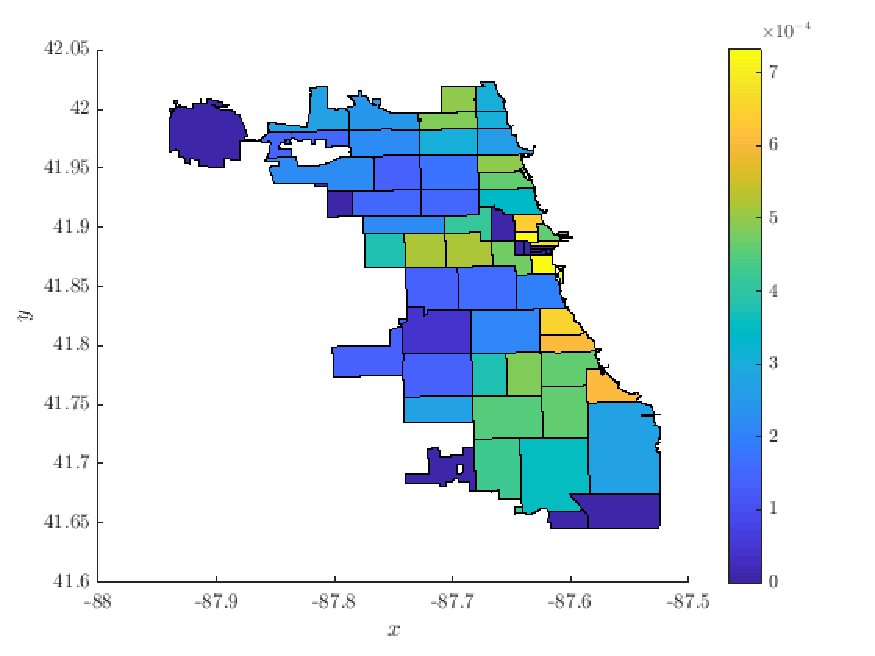
\includegraphics[width=\textwidth]{t0-cases}
				\caption{ZIP data.}
			\end{subfigure}%
			\begin{subfigure}{0.5\textwidth}
				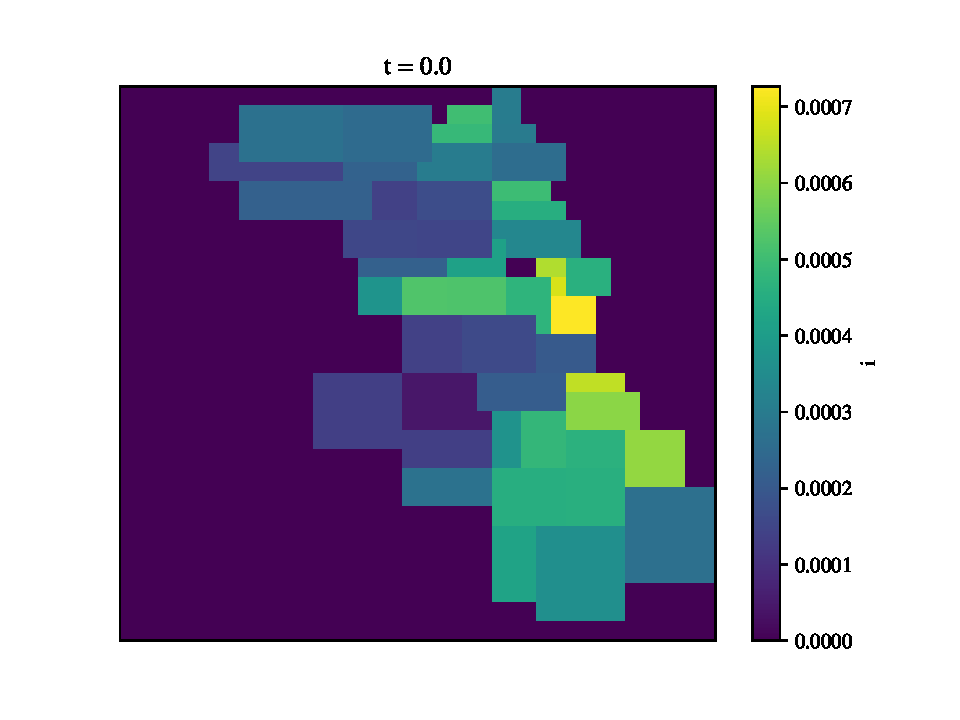
\includegraphics[width=\textwidth]{infected_0}
				\caption{Seeded model.}
			\end{subfigure}
			\caption{Initial seeding of the model with data from March 18, 2020.}
			\label{fig:seeding}
		\end{figure}
	
\section{Results}
	\subsection{Existence of solutions and basic reproduction numbers}
		We show that we are justified in searching for suitable parameters to solve the model.
		Let $\vec{x} = (S, A, I, R)$ and $\vec{x}_0 = (S_0, A_0, I_0, R_0)$.
		First we show that the solution of the initial value problem (\ref{eq:model}) exists for the case with no diffusion.
		\begin{theorem}
			Let $0 \leq \vec{x}_0 \leq 1$ be the initial datum.
			Then there exists a unique in time solution $\vec{x}$ of the initial value problem (\ref{eq:model}) without diffusion over $C \subset U \subset \R^4 \times \R^1$ where $C$ is a compact set that contains $(\vec{x}_0, t_0)$.
			Moreover, the solution is $\C^1$.
		\end{theorem}
		\begin{proof}
			Since $\vec{x}_t = f(\vec{x},t)$ is $\C^1$ on the open set $U \subset \R^4 \times \R^1$, it follows that there exists a solution of (\ref{eq:model}) without diffusion through the point $\vec{x}_0$ at $t = t_0$ for $|t - t_0|$ sufficiently small.
			Moreover, $\vec{x} (t, t_0,\vec{x_0})$ is a $\C^1$ function \cite{dynamics}.
			Since $C$ is a compact set containing $(\vec{x}_0, t_0)$, then the solution $\vec{x} (t, t_0, \vec{x}_0)$ can be uniquely extended backward and forward in $t$ up to the boundary of $C$ \cite{dynamics}.
		\end{proof}
		\noindent We do provide a proof for the existence of solutions to the initial boundary value problem (\ref{eq:model}) with diffusion terms, but we assume it exists.
		\begin{conjecture}
			Let $0 \leq \vec{x}_0 \leq 1$ the initial datum.
			Then there exists a unique global in time solution $\vec{x}$ of the initial boundary value problem (\ref{eq:model}).
		\end{conjecture}
		\noindent A proof for this conjecture will be similar to the one given in \cite{Mammeri+2020+102+113}.
		
		An important parameter in understanding the initial growth of the virus is the basic reproduction number.
		\begin{definition}[Basic Reproduction Number]
			The basic reproduction number $\Ro$ can be computed using the next generation of the model without diffusion.
			Since the infected individuals are in $A$ and $I$, new infections ($\mathcal{F}$) and transitions between compartments ($\mathcal{V}$) can be rewritten as
			\begin{align*}
				\mathcal{F} &= \begin{pmatrix} \omega (\beta_A A + \beta_I I) S \\ 0 \end{pmatrix}, &
				\mathcal{V} &= \begin{pmatrix} (\gamma_A + \delta) A \\ \gamma_I - \delta A \end{pmatrix}.
			\end{align*}
			Thus, $\Ro = \rho (\mat{F} \mat{V}^{-1})$ of the next generation matrix
			\begin{equation*}
				\mat{F} \mat{V}^{-1} = \begin{pmatrix} 
				\frac{S_0 \omega_0 \beta_A}{\gamma_A + \delta} + \frac{S_0 \omega_0 \beta_I \delta}{\gamma_I (\gamma_A + \delta)} & 
				\frac{S_0 \omega_0 \beta_I}{\gamma_I} \\ 
				0 & 0 \end{pmatrix}.
			\end{equation*}
			So,
			\begin{equation} \label{eq:ro}
				\Ro =  \frac{S_0 \omega_0}{\gamma_A + \delta}  \left( \beta_A + \beta_I \frac{\delta}{\gamma_I} \right).
			\end{equation}
		\end{definition}
		\noindent This number is dimensionless and has an epidemiological meaning.
		The first term represents the transmission rate by asymptomatic individuals, and the second term represents the transmission rate by symptomatic individuals.
			
	\subsection{Model resolution}
		Calibration of the model is done from March 18, 2020 to June 24, 2020.
		This range corresponds approximately to the first ``wave'' of cases seen in Chicago.
		The lockdown time points match exactly to the imposed lockdown of the city.
		That is, $t_\mathrm{bol} =$ March 21, 2020 and $t_\mathrm{eol} =$ May 29, 2020.
		In Figure \ref{fig:params}, the table shows the estimated parameters.
		Figure \ref{fig:fit} compares the data and the fitted symptomatic infected populations.
		\begin{figure}[h!]
			\centering
			\begin{subfigure}{0.55\textwidth}
				\begin{tabular}{c c c c}
					\hline
					$\omega_0 \beta_A$ & transmission rate due to $A$ & 0.1969 & days\textsuperscript{-1} \\
					$\omega_0 \beta_I$ & transmission rate due to $I$ & 0.3061 & days\textsuperscript{-1} \\
					$\eta$ & lockdown scale factor & 0.5514 & 1 \\
					$\delta$ & symptom onset rate & 0.0939 & days\textsuperscript{-1} \\
					$\gamma_A$ & removal rate of $A$ & 0.3632 & days\textsuperscript{-1} \\
					$\gamma_I$ & removal rate of $I$ & 0.1385 & days\textsuperscript{-1} \\
					\hline
				\end{tabular}
			\end{subfigure}%
			\begin{subfigure}{0.45\textwidth}
				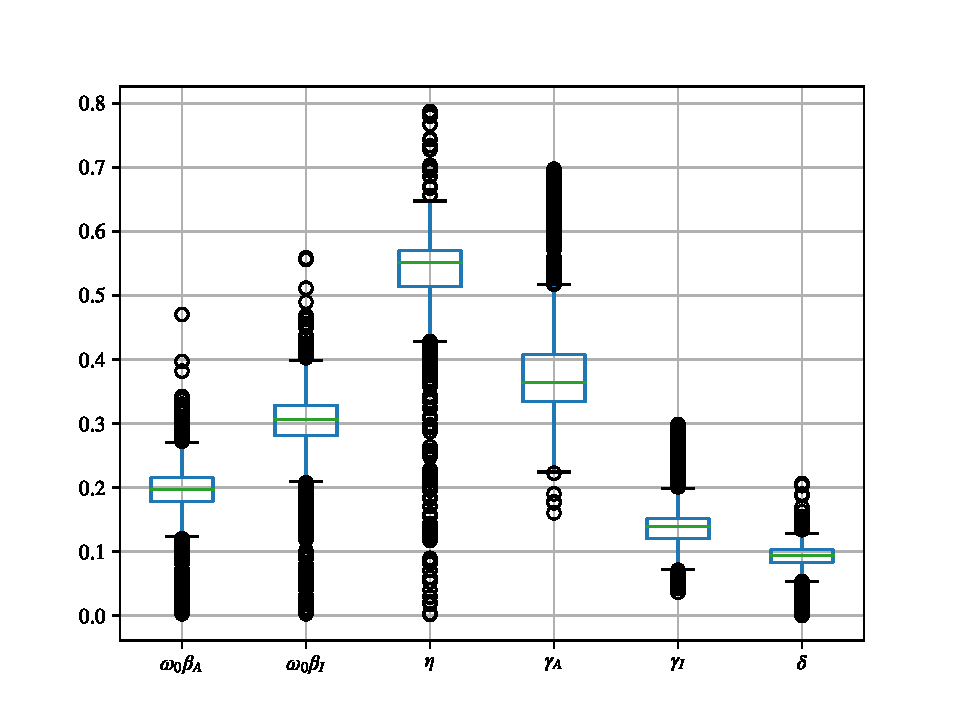
\includegraphics[width=\textwidth]{box-plot.pdf}
			\end{subfigure}
			\caption{Parameters calibrated according to data from the Chicago Data Portal.
				On the right is a boxplot of the parameter distribution from 1000 optimization iterations.}
			\label{fig:params}
		\end{figure}
	
		\begin{figure}[h!]
			\centering
			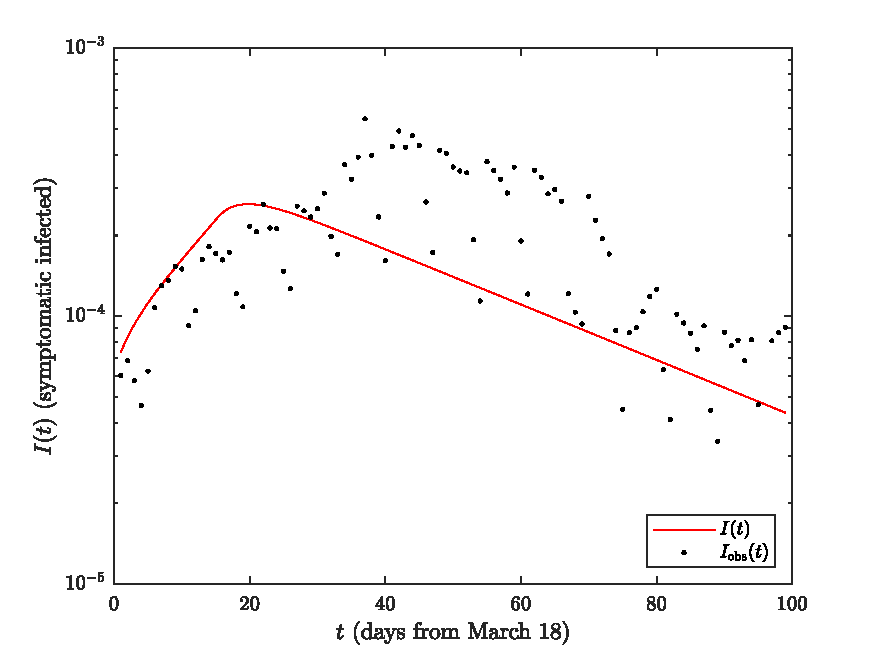
\includegraphics[width=0.5\textwidth]{cases.pdf}
			\caption{Fitting symptomatic infected by the median value.
				Note the logarithmic scale on the y-axis.}
			\label{fig:fit}
		\end{figure}
	
	\subsection{Spatial spread of COVID-19} \label{sec:spread}
		Simulations are performed from March 18, 2020 to June 24, 2020.
		The time step is $\Delta t = 0.2$ [days], chosen to satisfy the convergence condition \cite{pde}.
		
		Figure \ref{fig:spatial-results} presents three of the days from the simulation time: the effective lockdown $t_q$ day, the last day of simulation, and arbitrary day from the period in between.
		The observed data is shown on the left, while the model results are on the right.
		Comparing the model results to the data, we see that the model's diffusion mostly misses the diseases west-ward movement between days 15 and 35.
		Additionally, the model shows significantly fewer cases than are seen in the data (note the difference in the scale of the colorbars).
		
		In short, this model does not produce a reasonable reproduction of the spatial spread of COVID-19.
		\begin{figure}[H]
			\centering
			\begin{subfigure}{0.5\textwidth}
				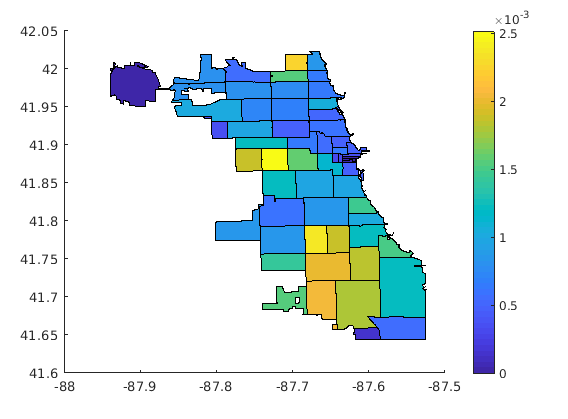
\includegraphics[width=\textwidth]{tq-cases}
				\caption{Observed Day 15 ($t_q$): April 2, 2020}
			\end{subfigure}%
			\begin{subfigure}{0.5\textwidth}
				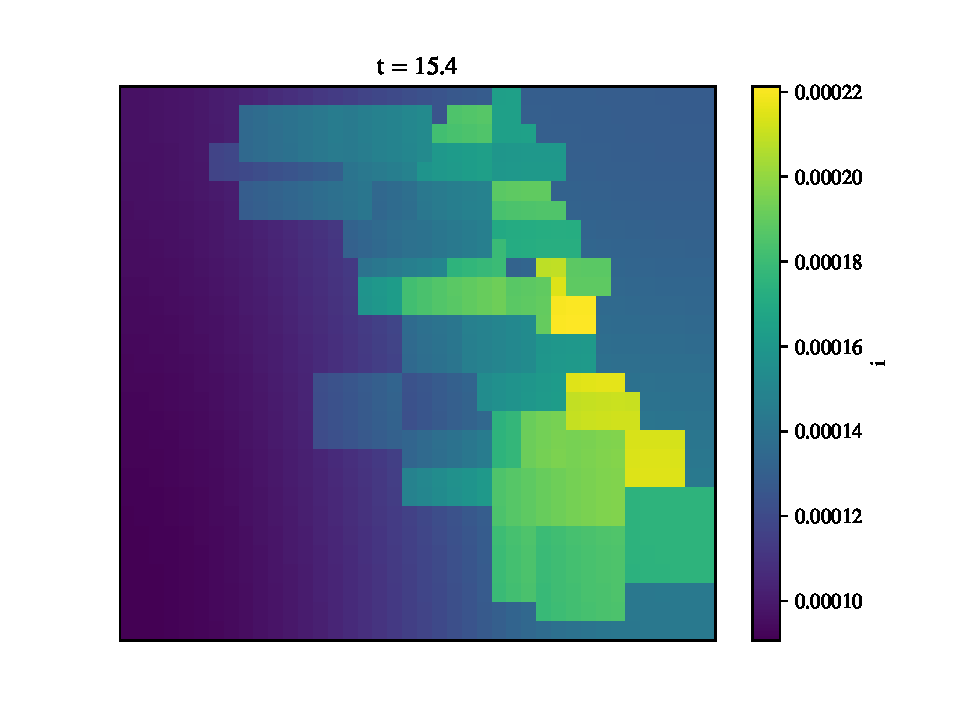
\includegraphics[width=\textwidth]{infected_15}
				\caption{Model Day 15 ($t_q$): April 2, 2020}
			\end{subfigure}
		
			\begin{subfigure}{0.5\textwidth}
				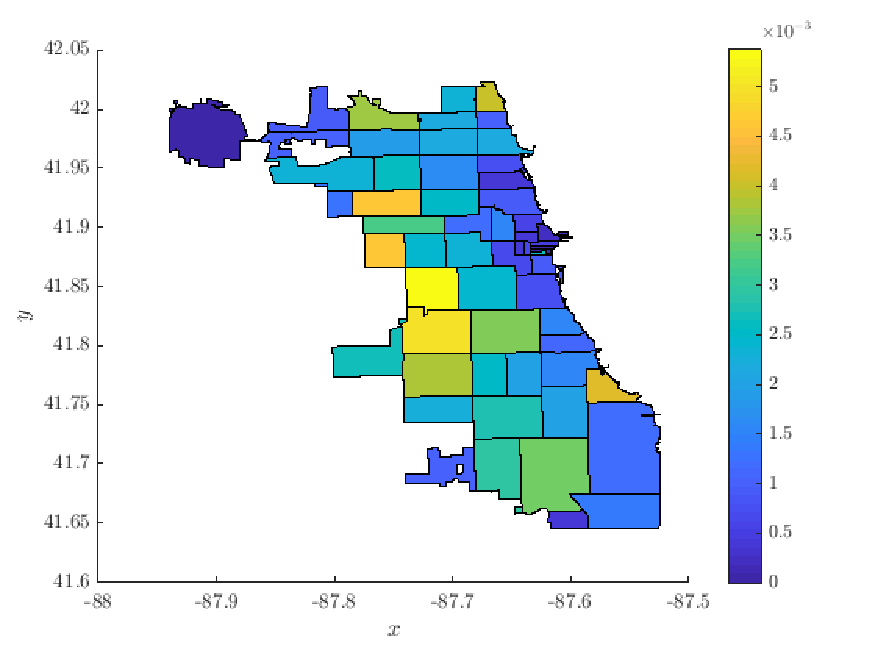
\includegraphics[width=\textwidth]{tmid-cases}
				\caption{Observed Day 35: April 22, 2020}
			\end{subfigure}%
			\begin{subfigure}{0.5\textwidth}
				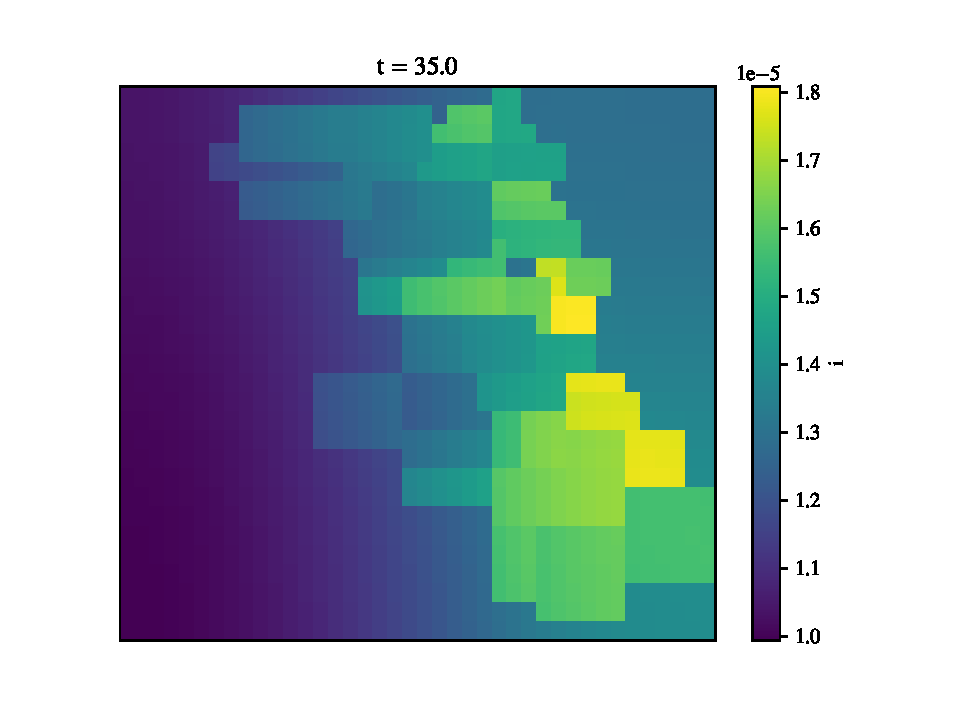
\includegraphics[width=\textwidth]{infected_35}
				\caption{Model Day 35: April 22, 2020}
			\end{subfigure}
		
			\begin{subfigure}{0.5\textwidth}
				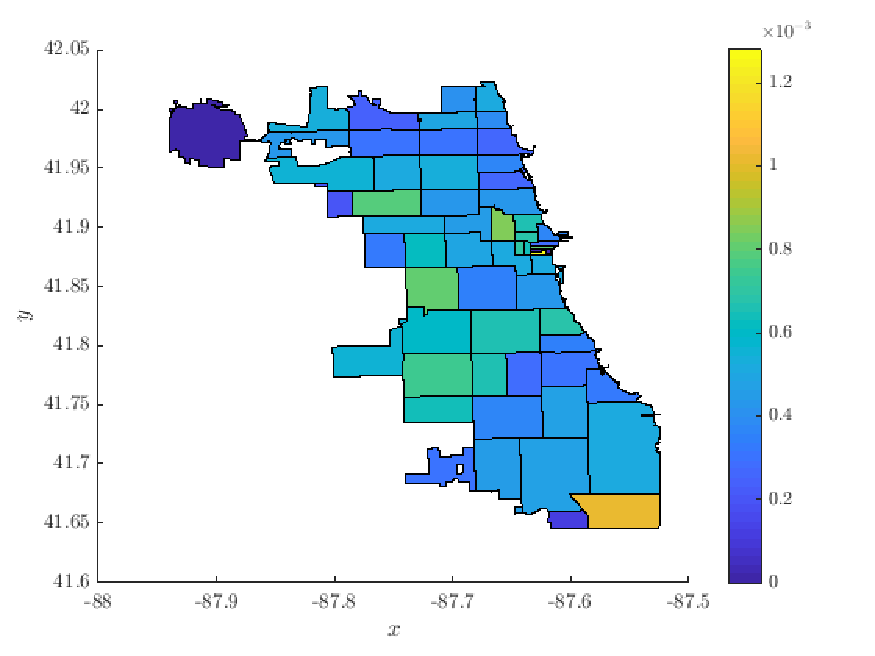
\includegraphics[width=\textwidth]{tfin-cases}
				\caption{Observed Day 99: June 24, 2020}
			\end{subfigure}%
			\begin{subfigure}{0.5\textwidth}
				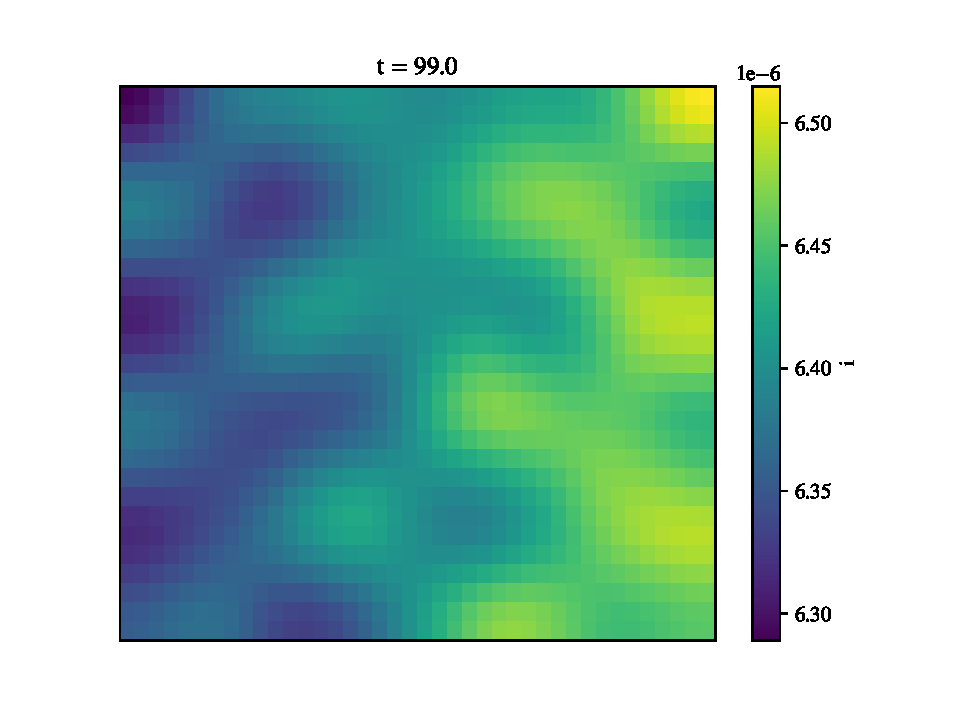
\includegraphics[width=\textwidth]{infected_99}
				\caption{Model Day 99: June 24, 2020}
			\end{subfigure}
		
			\caption{Comparison of observed infected cases and the model results.}
			\label{fig:spatial-results}
		\end{figure}
	

\section{Discussion}
	As mentioned in Section \ref{sec:spread}, the proposed model does not reproduce the spatial propagation of the virus.
	In this section, we address possible causes of these inaccuracies and discuss proposals for improving the results.
	
	The selected model populations may not, contrary to the assumption, be sufficient to describe the virus dynamics.
	Figure \ref{fig:fit} suggests this conclusion, since the growth of the model population only roughly describes the observed data.
	Note that after Day 20, the model and data begin to diverge substantially.
	This seems to correspond to the discrepancy in the number of cases seen in the spatial results in Figure \ref{fig:spatial-results}.
	Likely, the Exposed compartment describing the latent period is necessary, as in \cite{Mammeri+2020+102+113}.
	It is possible that the assumption that Deceased and Recovered populations can be modeled by the same population compartment is errant.
	On the other hand, in either case these populations have no effect on the act of transmission, so the model dynamics would likely be similar for both cases.
	A Deceased population may be useful for other reasons, as discussed below.
	
	The boundaries imposed on the computational domain (Equation \ref{eq:domain}) are likely not sufficient to force the diffusion process to replicate the true virus propagation.
	Figure \ref{fig:app-pops} shows the $S$ and $A$ populations at the same time points.
	There is a notable amount of diffusion of the $S$ population out of the boundaries of the city, including into Lake Michigan.
	Since the $S$ population diffuses into areas not reachable by the $I$ population, the reaction rates as described in Equation \ref{eq:model} are small.
	This may also explain the differences in case numbers seen in Figure \ref{fig:spatial-results}.
	It seems a tightening of the bounds of the computational domain is in order.
	Ideally, we would define the computational domain to be exactly the boundaries of the city.
	In practice, however, this is infeasible due to the irregularities of the shape.
	A better alternative is to define a polygon that approximates the shape of the city to be the computational domain.
	In any case, a new solver will be needed as the \verb|scikit-fdiff| module only allows rectangular domains.
	
	The optimization method can be improved in two ways.
	First, by adding a Deceased population we can modify the objective function (Equation \ref{eq:obj}) to compare both cases and deaths, as in \cite{Kevrekidis-2021}.
	COVID-19 death data is readily available, though requires caution to work with due to reporting inconsistencies.
	Second, we can perform the optimization directly on the spatial model, as in \cite{Mammeri+2020+102+113}, rather than relying on parameters from a temporal-only model.

\section*{Appendix}
	\subsection*{Nomenclature (Units are indicated in brackets.)}
		\begin{longtable}{c l l}
			\textbf{Latin symbols} & & \\
			$A$ & Asymptomatic infected individuals & [1] \\
			$D$ & Diffusivity & \\
			$I$ & Symptomatic infected individuals & [1] \\
			$J$ & Objective function & N/A \\
			$R$ & Removed individuals & [1] \\
			$\Ro$ & Basic reproduction number & [1] \\
			$S$ & Susceptible individuals & [1] \\
			\textbf{Greek symbols} & & \\
			$\beta_j$ & Contact rate of compartment $j$ & [days\textsuperscript{-1}] \\
			$\gamma_j$ & Recovery rate of compartment $j$ & [days\textsuperscript{-1}] \\
			$\Delta$ & Laplacian operator & N/A \\
			$\delta$ & Rate of asymptomatic individuals that may develop symptoms & [days\textsuperscript{-1}] \\
			$\eta$ & Lockdown scale factor & [1] \\
			$\theta$ & Parameter vector & N/A \\
			$\rho$ & Spectral radius & N/A \\
			$\Omega$ & Computational domain & N/A \\
			$\omega$ & Contacts & [1]
		\end{longtable}
	
	\newpage
	\subsection*{Model Populations}
		\begin{figure}[H]
			\centering
			\begin{subfigure}{0.5\textwidth}
				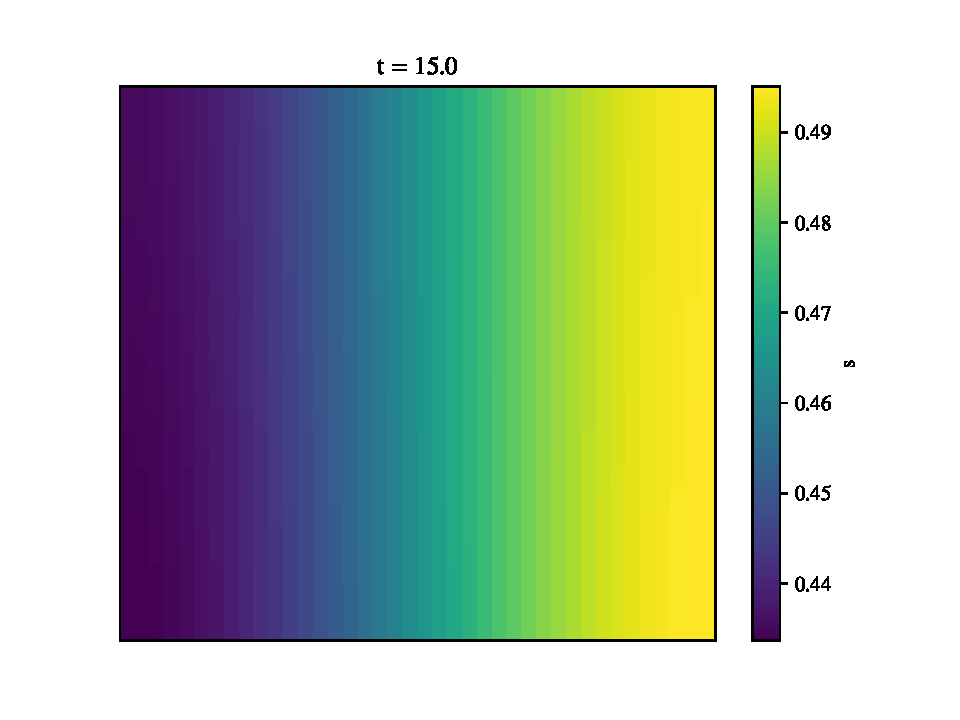
\includegraphics[width=\textwidth]{susceptible_15}
				\caption{Susceptible Day 15 ($t_q$): April 2, 2020}
			\end{subfigure}%
			\begin{subfigure}{0.5\textwidth}
				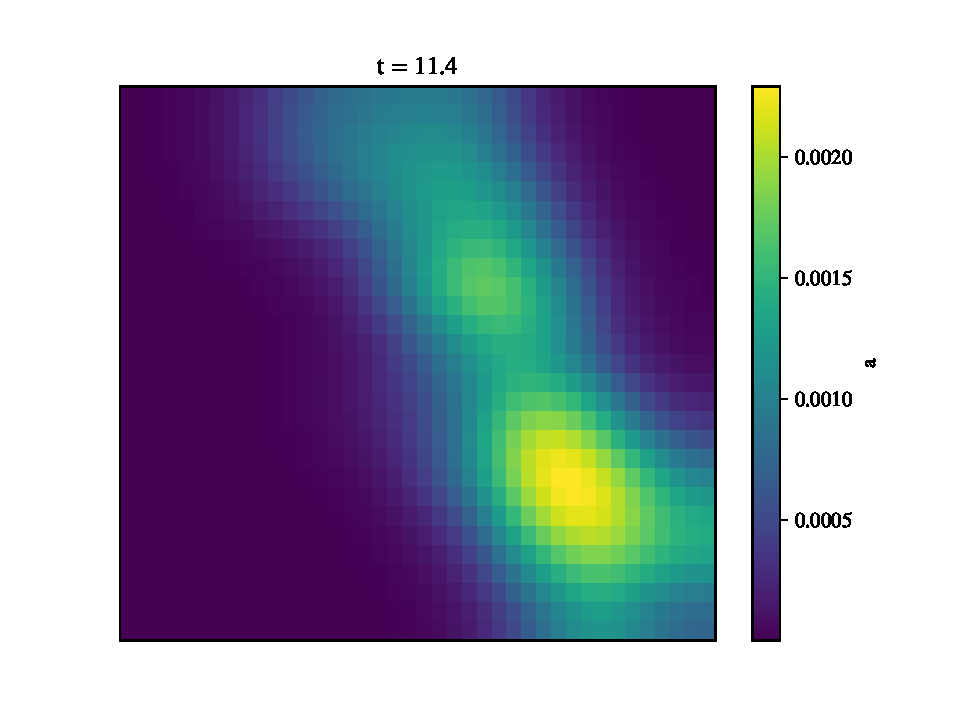
\includegraphics[width=\textwidth]{asymptomatic_15}
				\caption{Asymptomatic Day 15 ($t_q$): April 2, 2020}
			\end{subfigure}
			
			\begin{subfigure}{0.5\textwidth}
				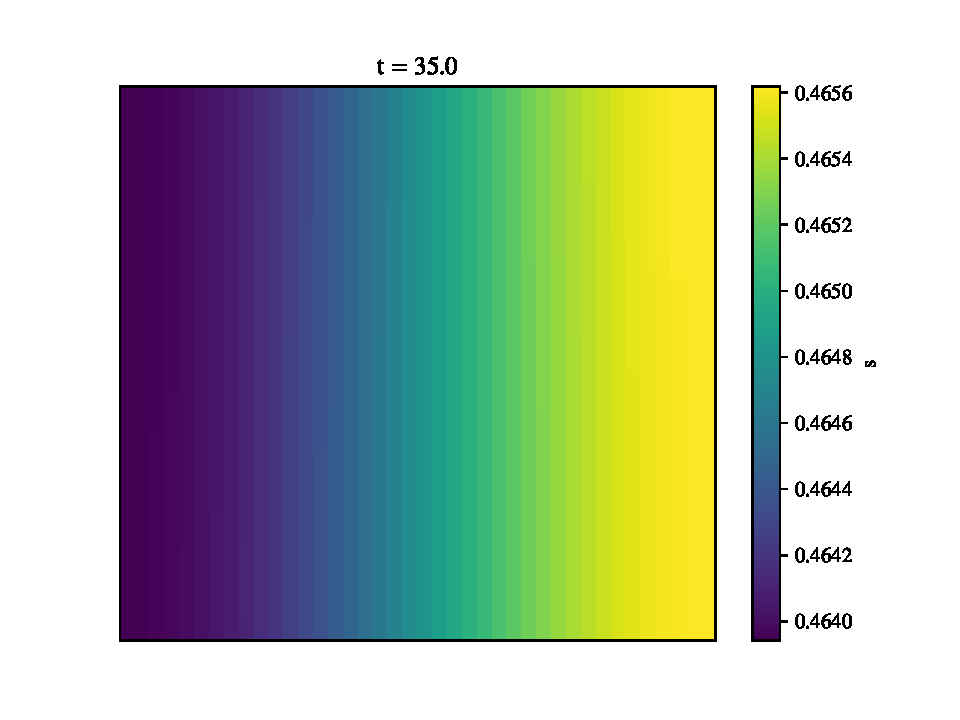
\includegraphics[width=\textwidth]{susceptible_35}
				\caption{Susceptible Day 35: April 22, 2020}
			\end{subfigure}%
			\begin{subfigure}{0.5\textwidth}
				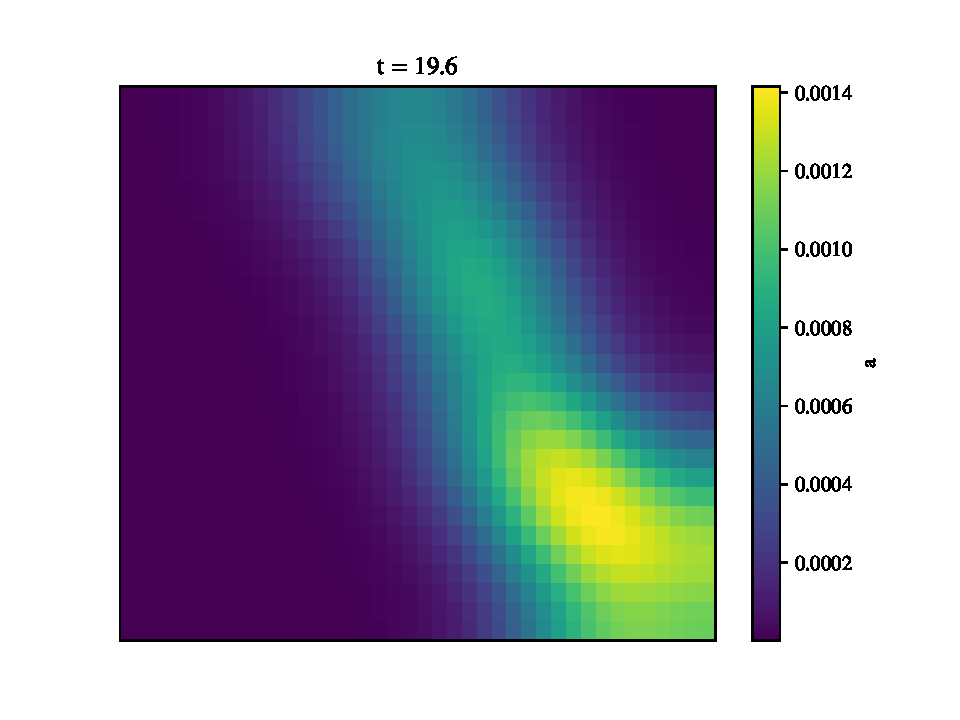
\includegraphics[width=\textwidth]{asymptomatic_35}
				\caption{Asymptomatic Day 35: April 22, 2020}
			\end{subfigure}
			
			\begin{subfigure}{0.5\textwidth}
				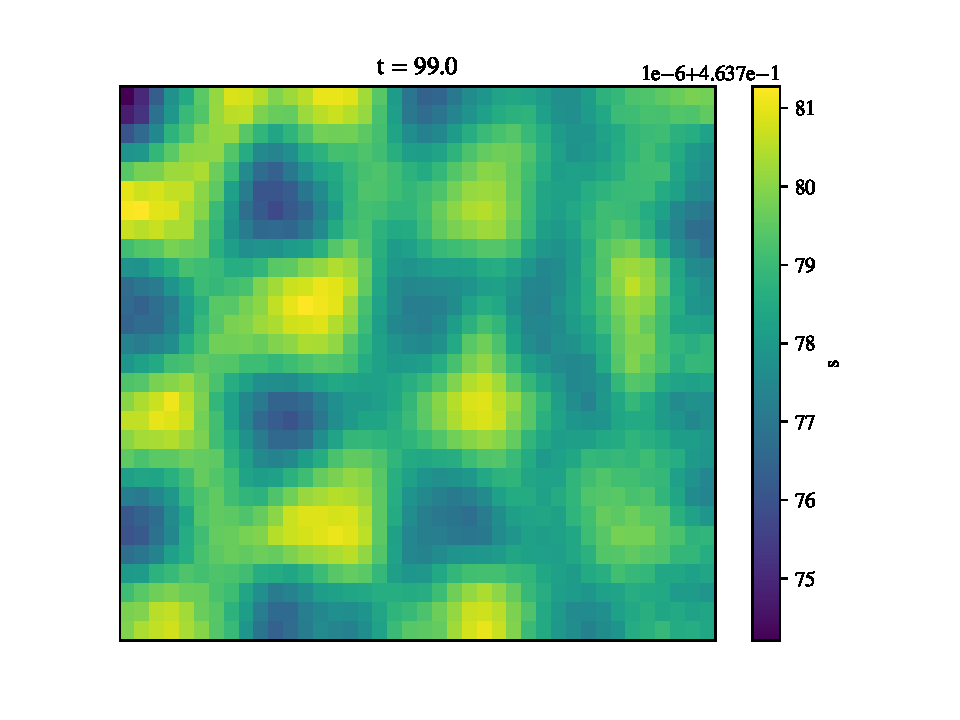
\includegraphics[width=\textwidth]{susceptible_99}
				\caption{Susceptible Day 99: June 24, 2020}
			\end{subfigure}%
			\begin{subfigure}{0.5\textwidth}
				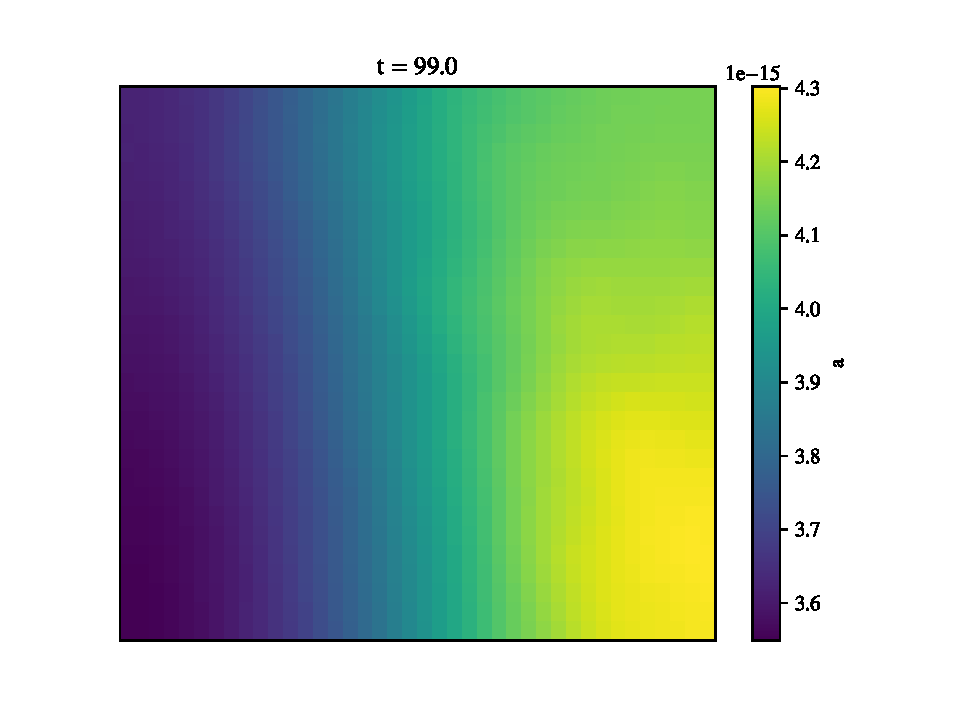
\includegraphics[width=\textwidth]{asymptomatic_99}
				\caption{Asymptomatic Day 99: June 24, 2020}
			\end{subfigure}
			
			\caption{Model results for susceptible and asymptomatic populations.}
			\label{fig:app-pops}
		\end{figure}

\bibliographystyle{abbrv}
\bibliography{version3}

\end{document}
